\documentclass[11pt,a4paper]{article}
% ---------------------------------------------------------------------------
% Shared preamble for the pitch-control calibration paper.
% ---------------------------------------------------------------------------
\usepackage[T1]{fontenc}
\usepackage[utf8]{inputenc}
\usepackage{lmodern}
\usepackage{microtype}
\usepackage[a4paper,margin=2.6cm]{geometry}
\usepackage{amsmath,amssymb}
\usepackage{graphicx}
\usepackage{booktabs}
\usepackage{multirow}
\usepackage{array}
\usepackage{tabularx}
\usepackage{enumitem}
\usepackage{xcolor}
\usepackage[labelfont=bf,font=small,labelsep=period]{caption}
\usepackage{tcolorbox}
\usepackage[round,authoryear]{natbib}
\usepackage[hidelinks,breaklinks]{hyperref}

\definecolor{ink}{HTML}{111111}
\definecolor{ink2}{HTML}{52514E}
\definecolor{rule1}{HTML}{2A78D6}
\definecolor{boxbg}{HTML}{F4F6F9}
\definecolor{boxline}{HTML}{C9D6E8}

\tcbset{
  plainstyle/.style={
    colback=boxbg, colframe=boxline, boxrule=0.5pt, arc=1.5pt,
    left=8pt, right=8pt, top=6pt, bottom=6pt,
    fonttitle=\bfseries\small, coltitle=ink
  }
}
\newtcolorbox{plainbox}[1][]{plainstyle, title={#1}}

% A short marginal-style aside that restates a technical point in ordinary words.
\newcommand{\plainly}[1]{%
  \par\smallskip\noindent\textcolor{rule1}{\rule{2.2pt}{9pt}}\hspace{5pt}%
  {\small\textit{In plain terms.} #1}\par\smallskip}

\setlength{\parskip}{0.35em}
\setlength{\tabcolsep}{5pt}
\renewcommand{\arraystretch}{1.12}

\captionsetup[table]{skip=4pt}
\captionsetup[figure]{skip=6pt}

\newcolumntype{R}{>{\raggedleft\arraybackslash}X}
\newcommand{\ci}[2]{\,\scriptsize[#1,\,#2]}


\title{\bfseries Sharp but Wrong:\\[0.25em]
\large Velocity-Free Pitch-Control Values Are Not Calibrated Probabilities}

\author{%
  \normalsize An evaluation against 137{,}545 realised ball arrivals\\
  \normalsize\itshape 179 matches, three competitions
}
\date{\normalsize\today}

\begin{document}
\maketitle
\thispagestyle{empty}

\begin{abstract}
\noindent
Pitch-control models return a number between zero and one for every point on the
football pitch, and that number is routinely described, and used, as the
probability that a team would control the ball if it arrived there. It is
multiplied by positional values to produce expected possession value, integrated
over regions to measure space creation, and compared against thresholds to
recommend passes. Each of those operations assumes the number is a calibrated
probability. We are not aware of any published test of that assumption, and the
apparent reason is that control is unobserved almost everywhere, which makes the
surface look unfalsifiable. It is not. Every pass, cross and clearance delivers
the ball somewhere, and at that point the model's value is an ordinary
probability forecast whose outcome is an ordinary draw. On 137{,}545 such
arrivals from 179 matches, we find that velocity-free pitch-control values are
not calibrated. A physics-based formulation discriminates well (AUC 0.762) yet
earns a Brier score of 0.167, nearly twice as bad as forecasting the base rate
everywhere (0.094); its calibration slope is 0.306, and a penalised logistic
regression given exactly the same state beats it by 0.089 Brier
(95\% CI 0.082 to 0.096). The error is five times larger in the attacking third
than the defensive third, grows monotonically with pass length, and is roughly
seven times larger on the destinations players choose least often. It transports
essentially unchanged across three competitions, including the men's-to-women's
boundary, so it is structural rather than local. It is also almost entirely
removable: a recalibration map fitted on two competitions strips 97--99\% of it
from a third. Downstream, aggregate possession value computed from raw control
values is 28\% lower than from calibrated ones, and 36\% of threshold-based pass
recommendations change. The ordering these models produce is sound; the numbers
attached to that ordering are not.
\end{abstract}

\vspace{0.6em}

\begin{plainbox}[Scope --- stated before anything else]
\small
This paper evaluates the \textbf{velocity-free, camera-limited} variants of three
pitch-control formulations on freeze-frame data. A freeze frame is a single
snapshot, so no model here has access to player velocity, and the camera records
a median of 16 of the 22 players. \textbf{This is not a test of published
full-tracking pitch-control models.} It is a test of what those formulations do
under the data conditions most clubs and researchers outside the elite tier
actually work with --- a different question, and one the results suggest is worth
answering on its own terms. Section~\ref{sec:limits} returns to this at length.

All results are reproducible from \texttt{scripts/} on data obtainable with
\texttt{scripts/fetch\_data.py}. No number in this paper was chosen after seeing
the data: the hypotheses, subgroups, horizons and metrics were fixed in the
project's proposal beforehand, and the analysis order is frozen in code.
\end{plainbox}

\clearpage
\tableofcontents
\clearpage

% ===========================================================================
\section{A plain-language summary}
% ===========================================================================

This section is written for a reader who does not work in sports analytics. The
rest of the paper assumes some statistics; this part does not.

\paragraph{What a pitch-control model does.}
Give it a photograph of a moment in a football match --- where all twenty-two
players are standing --- and it colours in the whole pitch. Each point gets a
number between 0 and 1. Red means ``if the ball went here, the attacking team
would end up with it''; blue means the defending team would. Panel~(a) of
Figure~\ref{fig:concept} is one of these pictures, computed from a real frame.

\paragraph{What the number is supposed to mean.}
If the model writes 0.7 on a patch of grass, and it is behaving like a
probability, then across all the times it writes 0.7, the attacking team should
end up with the ball about seven times in ten. Panel~(b) of
Figure~\ref{fig:concept} shows what that commitment looks like. This is a strong
claim, and it is the one every downstream use of these models relies on: you
cannot multiply a number by the value of a location, or add it up across a
season, unless it is on a real probability scale.

\paragraph{Why nobody had checked.}
The colours cover the whole pitch, and the ball only goes to one place. Most of
the picture describes something that never happened, so it looks untestable. But
the part that \emph{did} happen is testable: every pass lands somewhere. Take the
model's number at the spot where the ball actually arrived, then look at what
actually happened next. Do that for 137{,}545 arrivals and you have an ordinary
forecast-verification problem --- the same problem weather forecasters solved
half a century ago when they asked whether ``70\% chance of rain'' meant
anything.

\paragraph{What we found.}
The models are good at ranking and bad at scale. They reliably say a higher
number for situations where the attacking team is more likely to keep the ball
--- that part works. But the numbers themselves are wrong, and wrong in a
consistent direction. When the physics-based model says 0.4, the ball is in fact
kept about eight times in ten (Figure~\ref{fig:reliability}). Its overall score
is worse than if it had ignored the players entirely and guessed the same number
every time (Figure~\ref{fig:decomposition}). The error is worst exactly where
these models get used most: in front of goal, and on long passes
(Figure~\ref{fig:breaks}).

\paragraph{What it costs, and what fixes it.}
Because possession-value calculations multiply by these numbers, the error does
not wash out --- it compounds. Aggregate possession value comes out 28\% too low,
and about a third of ``should I play this pass?'' recommendations flip
(Figure~\ref{fig:downstream}). The repair is mundane: one correction curve,
fitted once on two competitions, removes 97--99\% of the problem on a third
(Figure~\ref{fig:transport}). Two or three numbers, fitted once, and the field
becomes usable for the arithmetic people were already doing with it.

\begin{figure}[t]
  \centering
  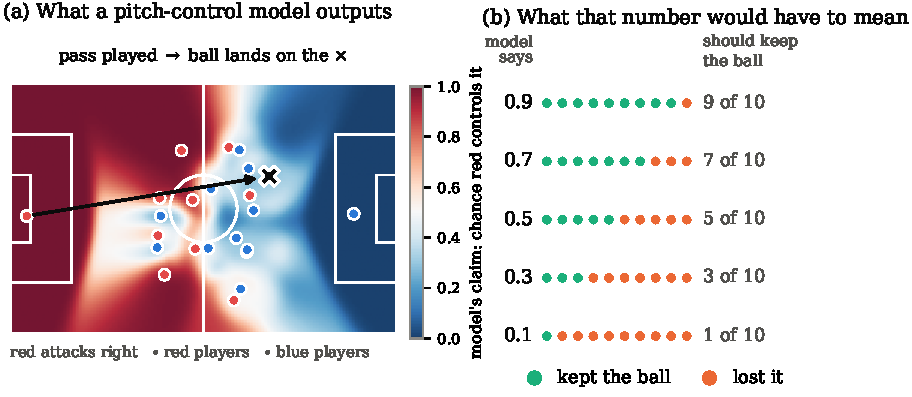
\includegraphics[width=\textwidth]{figures/fig01_concept.pdf}
  \caption{\textbf{What a pitch-control model outputs, and what it would have to
  mean.} (a)~A control surface computed from a real freeze frame: red is the
  attacking team's claim on each point, blue the defending team's. The arrow is
  the pass that was actually played; the cross is where the ball arrived. Only
  the value at the cross is ever tested against an outcome. (b)~What it means for
  the number to be a probability rather than a shading: across all the arrivals
  where the model says 0.7, the attacking team should keep the ball about seven
  times in ten.}
  \label{fig:concept}
\end{figure}

% ===========================================================================
\section{Introduction}
% ===========================================================================

A pitch-control model takes the instantaneous positions of the players and
returns a field over the pitch,
\[
  C_A(x, y, t) \in [0, 1],
\]
routinely described as the probability that team~$A$ would control the ball were
it to arrive at point $(x, y)$ at time~$t$. The number is not merely displayed.
It is multiplied by positional values to produce expected possession value,
integrated over regions to produce space-creation metrics, differenced across
counterfactual player positions to value off-ball runs, and compared against
thresholds to recommend passes \citep{fernandez2018wide, fernandez2021epv,
spearman2018beyond}. Every one of those operations presupposes that $C_A$ is a
calibrated probability.

That presupposition has, as far as we can establish, not been tested. We are not
aware of a published reliability diagram or proper-scoring-rule decomposition for
any pitch-control model. The apparent obstacle is counterfactuality: control is
unobserved at almost every point on the pitch, so the field looks unfalsifiable.

It is not. At every pass, cross and clearance the ball genuinely arrives
somewhere, and at that point the model's value is an ordinary probability
forecast whose outcome is an ordinary draw. A season of data supplies tens of
thousands of such forecast--outcome pairs. What follows is a standard
probabilistic forecast evaluation, using apparatus settled in meteorology fifty
years ago \citep{brier1950verification, murphy1973partition} and not, to our
knowledge, previously applied here.

\subsection*{Contributions}

\begin{enumerate}[leftmargin=1.4em, itemsep=0.25em]
  \item The first calibration assessment of pitch-control models we are aware of,
        on 137{,}545 arrivals across 179 matches and three competitions.
  \item A demonstration that discrimination and calibration diverge sharply in
        this domain: the physics-based model ranks situations well
        (AUC~0.762) while scoring \emph{worse than forecasting the base rate}.
  \item A characterisation of where the error concentrates --- the attacking
        third, long passes, poorly observed frames --- and evidence that it is
        structural rather than local, transporting unchanged across competitions
        and across the men's/women's boundary.
  \item Evidence that the defect is repairable: a recalibration map fitted on two
        competitions removes 97--99\% of the measured miscalibration on a third.
  \item Quantification of the downstream consequence: aggregate possession value
        is understated by 28\%, and 36\% of threshold-based pass recommendations
        change under recalibration.
  \item A tested, open implementation of the whole protocol, including adapters
        for three providers and an instrument-validation suite.
\end{enumerate}

% ===========================================================================
\section{Why a good AUC does not make a good probability}
\label{sec:auc}
% ===========================================================================

The single most important technical point in this paper is that two desirable
properties of a forecast are independent, and the sports-analytics literature
routinely reports only one of them.

\textbf{Discrimination} asks whether the forecast \emph{orders} cases correctly:
do the situations that turned out well receive higher numbers than the ones that
turned out badly? The area under the ROC curve (AUC) measures exactly this and
nothing else.

\textbf{Calibration} asks whether the numbers themselves are right: among all the
cases assigned 0.7, did roughly 70\% turn out well?

AUC is invariant to any strictly increasing transformation of the forecast.
Replace every forecast $p$ by $p^{3}$, or by $0.5p + 0.25$, and the AUC does not
move by a single decimal place --- while the probabilities become arbitrarily
wrong. Figure~\ref{fig:auc} makes this concrete on our own data: applying an
isotonic recalibration map changes every forecast value substantially, leaves the
ordering untouched, and leaves the AUC identical to three decimal places.

\plainly{AUC is a test of who you rank first. Calibration is a test of what the
number means. A model can win the first test and fail the second completely, and
reporting only AUC is how a field ends up with numbers that look like
probabilities and do not behave like them.}

\begin{figure}[t]
  \centering
  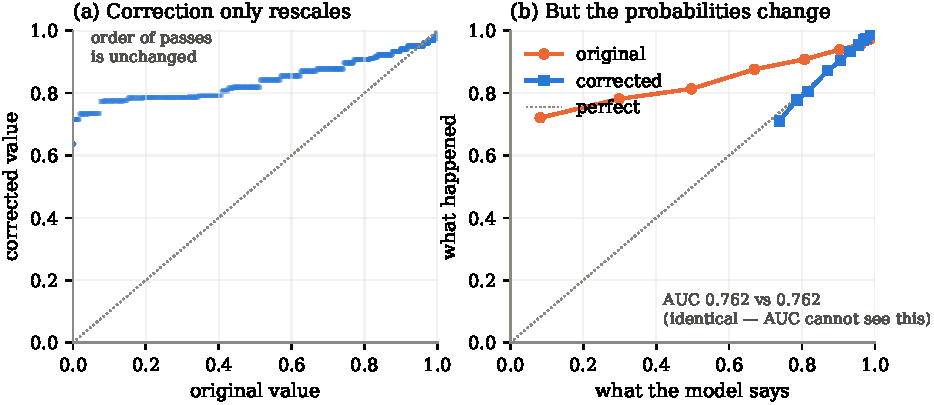
\includegraphics[width=\textwidth]{figures/fig02_calibration_vs_discrimination.pdf}
  \caption{\textbf{A correction that changes every probability and no rankings.}
  (a)~Each point is one arrival: its original forecast against its corrected one.
  The mapping is increasing everywhere, so no pass overtakes another. (b)~The two
  versions plotted against what actually happened. The corrected forecasts sit on
  the diagonal, the originals far above it --- and the AUC is identical
  (0.762 versus 0.762). A discrimination metric cannot see the difference between
  these two panels.}
  \label{fig:auc}
\end{figure}

We take the standard position that a forecast should be
\emph{sharp subject to being calibrated} \citep{gneiting2007sharpness}:
calibration is the constraint, and informativeness is what one maximises within
it. A forecast that is merely sharp --- confident, spread towards 0 and 1 --- is
not thereby good, and the results below show a family of models that are very
sharp and badly miscalibrated.

% ===========================================================================
\section{Related work}
% ===========================================================================

Dominant-region models partition the pitch by which player reaches each point
first \citep{taki2000dominant, fujimura2005geometric}. Physics-based
formulations make arrival time uncertain and let control accumulate dynamically
\citep{spearman2017physics, spearman2018beyond}; related space-occupation and
possession-value work embeds such surfaces in full valuation frameworks
\citep{fernandez2018wide, fernandez2021epv}. \citet{brefeld2019zones} learn
movement models from data and derive zones of control from them --- the closest
existing work to a statistically grounded control field. A broader survey of
spatio-temporal football analysis is given by \citet{gudmundsson2017survey}.

None of this literature reports whether the resulting values behave like
probabilities. The apparatus for asking exists and is mature: proper scoring
rules \citep{brier1950verification, gneiting2007proper}, the
sharpness-subject-to-calibration framing \citep{gneiting2007sharpness}, score
decompositions \citep{murphy1973partition}, the calibration hierarchy
\citep{vancalster2016hierarchy, vancalster2019achilles}, and binning-free
reliability diagrams via isotonic regression \citep{dimitriadis2021corp}.
Recalibration is equally well established \citep{platt1999probabilistic,
zadrozny2002isotonic, kull2017beta}, as is the critique of binned calibration
error \citep{nixon2019measuring, kumar2019verified, vaicenavicius2019evaluating,
roelofs2022mitigating}.

The contribution here is a transfer, not an invention. Full references, with
unverified bibliographic details explicitly flagged, are in
\texttt{docs/references.bib}.

% ===========================================================================
\section{Problem formulation}
% ===========================================================================

\subsection{Three constructs, routinely conflated}

Reachability (``who gets there first'') is a question about locomotion.
Possession (``who ends up with the ball'') adds the contest at the point of
contact. Retention (``who still has it after the next action'') adds the quality
of the subsequent decision. These are different quantities, and in aggregate
\[
  C^{\mathrm{reach}} \;\geq\; C^{\mathrm{possess}} \;\geq\; C^{\mathrm{retain}}.
\]
Dominant-region models compute the first. The probabilistic reading used
downstream asserts the second. We evaluate against the second, and return to the
resulting objection in Section~\ref{sec:limits}.

\subsection{Operational definition of the outcome}

\begin{plainbox}[The label]
\small
$Y = 1$ if and only if a player of team~$A$ is in possession at
$t_{\mathrm{arrival}} + h$, with $h = 1.0$\,s. Arrivals whose horizon window is
interrupted by a stoppage are \textbf{censored and excluded}, not counted as
failures.
\end{plainbox}

Censoring rather than coding stoppages as losses avoids biasing every model
downward in the zones where fouls concentrate. It is not free: censoring is
itself selective, and the censored fraction is reported throughout.
Section~\ref{sec:construct} sweeps $h$ and three alternative outcome definitions
to show the conclusion does not depend on this choice.

\subsection{The estimand}

A model is calibrated on a population of arrivals if
\[
  \mathbb{E}\!\left[\,Y \,\middle|\, C_A(X) = c\,\right] = c
  \qquad\text{for almost every } c \text{ in the support of the forecast.}
\]
This is \emph{weak} calibration in the hierarchy of
\citet{vancalster2016hierarchy} --- conditioning on the forecast value, not on
the full covariate vector. Strong calibration is not testable at realistic sample
sizes and is not claimed.

\subsection{Selection}

The ball arrives only where someone sent it. Writing $D = 1$ for an observed
arrival, the data identify $P(Y \mid X, D = 1)$ while the field claims to
describe $P(Y \mid X)$. These coincide only if $Y \perp\!\!\!\perp D \mid X$. Two
obstacles separate them: covariate shift in where the ball goes, which
reweighting can in principle address \citep{horvitz1952generalization,
quinonero2009dataset}, and selection on what the passer knew and the state vector
does not contain, which it cannot. Section~\ref{sec:selection} treats both, and
reports that the reweighting arm failed its own diagnostics.

% ===========================================================================
\section{Data}
% ===========================================================================

\subsection{Corpus}

We use 179 matches of StatsBomb~360 freeze-frame data across three competitions.
151{,}418 ball arrivals were extracted and 137{,}545 retained after the
pre-registered inclusion criteria, of which 40{,}867 fall in the test fold across
53 held-out matches.

\begin{table}[h]
\centering
\small
\caption{The corpus. ``Base rate'' is the share of arrivals after which the
attacking team is in possession one second later.}
\label{tab:corpus}
\begin{tabular}{lrrr}
\toprule
Competition & Matches & Arrivals & Base rate \\
\midrule
FIFA World Cup 2022     & 64 & 51{,}390 & 0.909 \\
UEFA Euro 2024          & 51 & 42{,}077 & 0.921 \\
Women's World Cup 2023  & 64 & 44{,}078 & 0.859 \\
\bottomrule
\end{tabular}
\end{table}

\subsection{What the data does and does not contain}

The following were verified against the files themselves rather than taken from
documentation:

\begin{itemize}[leftmargin=1.4em, itemsep=0.2em]
  \item \textbf{Flight time is measured}, not imputed: every pass carries a
        duration, with implied ball speeds of 6.9--22.1\,m/s (median 13.1).
  \item \textbf{Possession is labelled at event level}, so the outcome is not
        reconstructed from a transfer log.
  \item \textbf{There is no velocity.} A freeze frame is one snapshot.
  \item \textbf{The camera limits what exists.} 360 frames cover 83.9\% of
        passes; the median pass event shows 16 of 22 players; all 22 are visible
        at roughly 1 arrival in 2{,}500; and \textbf{21\% of pass destinations
        fall outside the \texttt{visible\_area} polygon}, where ``no defender
        near the destination'' means ``no defender visible''.
  \item \textbf{No exogenous arrivals.} Only pass events carry both a start and
        an end location, so the corpus contains no deflections, clearances or
        second balls. This removes the strongest available identification
        strategy against selection (Section~\ref{sec:selection}).
\end{itemize}

The derived outcome agrees with the provider's own pass outcome on 96.6\% of
completed passes. On incomplete passes the two diverge --- roughly half of failed
passes still end with the same team in control a second later --- which is the
construct distinction above made visible rather than an error.

\subsection{Dependence}

Arrivals cluster within matches. The measured intra-match ICC is 0.013 and the
\textbf{design effect is 11.1}, so intervals computed as though arrivals were
independent would be about 3.3 times too narrow. All intervals below are
percentile cluster bootstraps over 1{,}000 replicates resampling whole matches
\citep{cameron2015cluster, efron1993bootstrap}.

\plainly{Two passes from the same match are not two independent pieces of
evidence --- the same teams, pitch and referee produced both. Treating them as
independent would make our error bars roughly three times narrower than they
should be, so we resample whole matches instead of individual passes.}

% ===========================================================================
\section{Methods}
% ===========================================================================

\subsection{Models}

All models receive identical information and are evaluated on identical
arrivals. The point of including fitted baselines is not to propose a better
pitch-control model; it is to establish what is achievable from the same state
vector, so that the unfitted models' scores can be read against something other
than zero.

\begin{table}[h]
\centering
\small
\caption{The six models. Only M0, M3 and M4 see the outcome during fitting;
M2a fits a single scale parameter.}
\label{tab:models}
\begin{tabularx}{\textwidth}{llX}
\toprule
& Fitted? & Description \\
\midrule
\textbf{M0} Base rate & yes & Predicts the training base rate everywhere.
  Perfectly calibrated, useless; the reference for resolution. \\
\textbf{M1} Voronoi & no & $C_A = \mathbf{1}[\min_j \tau_j < \min_k \tau_k]$.
  Hard 0/1 output. \\
\textbf{M2} Physics & no & Logistic arrival times with competing-risks
  accumulation of control. Parameters ($\sigma$, $\lambda$, $v_{\max}$, $t_r$)
  assumed, not estimated. \\
\textbf{M2a} Reachability sigmoid & one parameter &
  $C_A = \sigma\!\left((\min_k \tau_k - \min_j \tau_j)/s\right)$. Isolates how
  much of M2 is a monotone squash of a time-to-point difference. \\
\textbf{M3} Logistic & yes & Penalised logistic regression on engineered
  kinematic features computed from exactly the state M1/M2 receive. \\
\textbf{M4} GBM & yes & Histogram gradient boosting on the same features. \\
\bottomrule
\end{tabularx}
\end{table}

\subsection{Evaluation}

Splits are by \textbf{match}, never by row: arrivals nest within possessions
within matches, and a random split rewards memorising a match's shape.
Recalibration maps are fitted on a validation fold disjoint from both the fitting
and test data; the protocol raises an error if a split lacks one. A leakage audit
is written with every run.

The primary calibration statistic is the \textbf{match-cross-fitted CORP
miscalibration term} (MCB) of the Brier score \citep{dimitriadis2021corp}, not
binned expected calibration error. The CORP construction decomposes the Brier
score as
\[
  \mathrm{BS} \;=\; \mathrm{MCB} \;-\; \mathrm{DSC} \;+\; \mathrm{UNC},
\]
where MCB is the penalty for the probabilities being on the wrong scale, DSC is
the credit for carrying information about which arrivals differ, and UNC is the
irreducible difficulty of the question (the variance of the outcome). The
reference forecast is obtained by pool-adjacent-violators isotonic regression
rather than by binning.

We avoid binned ECE deliberately: it depends on an arbitrary bin count, is
biased, is not a proper scoring rule, and can be driven near zero by coarsening
\citep{nixon2019measuring, kumar2019verified}. Our test suite constructs a
forecast whose two-bin ECE is under 0.02 and whose forty-bin ECE exceeds 0.08.
One caveat of the CORP estimator matters here and is handled explicitly: in
sample, MCB is biased \emph{upward}, because the isotonic fit absorbs noise. We
therefore cross-fit by match, and we do not truncate negative estimates.

\plainly{MCB is ``how much of the score is wasted on the numbers being on the
wrong scale''. Zero means the probabilities mean what they say. It is the single
number this paper is about, and throughout the figures it is labelled simply
``size of the error''.}

\subsection{Instrument validation}

Before measuring anything, the calibration estimator was validated against a
known ground truth on simulated data. It reports near-zero miscalibration for an
oracle forecast; recovers an injected logit distortion to within 0.01 of the
injected slope; confirms that AUC is unchanged to machine precision by that
distortion; and produces intervals 2.3 times wider under clustering than a naive
bootstrap. All eight checks pass and are re-run by
\texttt{scripts/09\_validate\_instrument.py}.

This step is worth naming explicitly. A calibration finding is a claim about an
instrument as much as about a model, and an uncalibrated instrument would produce
exactly the paper we did not want to write.

% ===========================================================================
\section{Results}
% ===========================================================================

Test fold: 40{,}867 arrivals across 53 held-out matches, base rate 0.894.

\subsection{Overall calibration}

\begin{table}[h]
\centering
\small
\caption{Headline results on the held-out fold. Brackets are 95\% percentile
cluster-bootstrap intervals over 1{,}000 match resamples. Forecast SD is the
standard deviation of the model's output --- a measure of how confident it is.}
\label{tab:headline}
\begin{tabular}{lccccccc}
\toprule
Model & Brier & 95\% CI & MCB & DSC & Slope & AUC & Forecast SD \\
\midrule
M1 Voronoi          & 0.231 & [0.216, 0.244] & 0.142 & 0.006 & 0.114 & 0.675 & 0.428 \\
M2 Physics          & 0.167 & [0.156, 0.177] & \textbf{0.081} & 0.008 & \textbf{0.306} & 0.762 & 0.313 \\
M2a Reach.\ sigmoid & 0.155 & [0.146, 0.163] & 0.069 & 0.008 & 0.636 & 0.761 & 0.247 \\
M0 Base rate        & 0.094 & [0.088, 0.101] & 0.000 & 0.000 & ---   & 0.500 & 0.000 \\
M3 Logistic         & 0.078 & [0.072, 0.084] & 0.001 & 0.017 & 1.014 & 0.837 & 0.133 \\
M4 GBM              & 0.073 & [0.068, 0.079] & 0.000 & 0.021 & 1.018 & 0.864 & 0.145 \\
\bottomrule
\end{tabular}
\end{table}

\noindent
The MCB interval for M2 is [0.075, 0.087]; for M1, [0.133, 0.152]; for M2a,
[0.064, 0.073]. None of them contains zero.

The unfitted geometric models are not calibrated. The physics model's calibration
slope of 0.306 is the signature of severe overconfidence in scale: the forecast
spreads towards 0 and 1 roughly three times further than the evidence supports.
Its mean forecast is 0.72 against a base rate of 0.89, so it also under-forecasts
systematically. Figure~\ref{fig:reliability} shows this directly.

\begin{figure}[t]
  \centering
  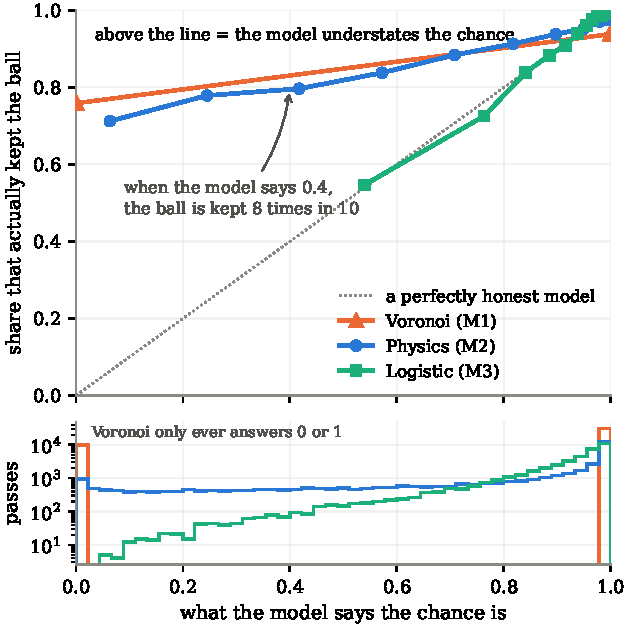
\includegraphics[width=0.66\textwidth]{figures/fig03_reliability.pdf}
  \caption{\textbf{Reliability of three models on the held-out fold.} A perfectly
  honest model would trace the dotted diagonal. The two unfitted models sit well
  above it --- they understate the attacking team's chances by 0.14 (Voronoi) and
  0.17 (physics) on average --- while the fitted logistic lies on it to within
  0.001. The lower panel shows how often each value is actually emitted; the
  physics model spends most of its output range in a region where its numbers are
  badly wrong, and the Voronoi model emits nothing but 0 and 1.}
  \label{fig:reliability}
\end{figure}

\begin{plainbox}[The central observation of this paper]
\small
M2 discriminates well --- AUC 0.762, far above chance --- while scoring 0.167 on
the Brier score, nearly twice as bad as forecasting the base rate everywhere
(0.094). \textbf{A model that looks good on a discrimination metric can be worse
than useless as a probability.} M0 makes the converse point: it is perfectly
calibrated (MCB 0.000) and carries no information whatever (DSC 0.000,
AUC 0.500). Neither property substitutes for the other.
\end{plainbox}

Figure~\ref{fig:decomposition} shows where each model's score goes. The grey
segment is the difficulty of the question, identical for every model; the green
segment is the credit a model earns for being informative; the orange segment is
the penalty it pays for being on the wrong scale. For M1, M2 and M2a the penalty
dwarfs the credit by an order of magnitude.

\begin{figure}[t]
  \centering
  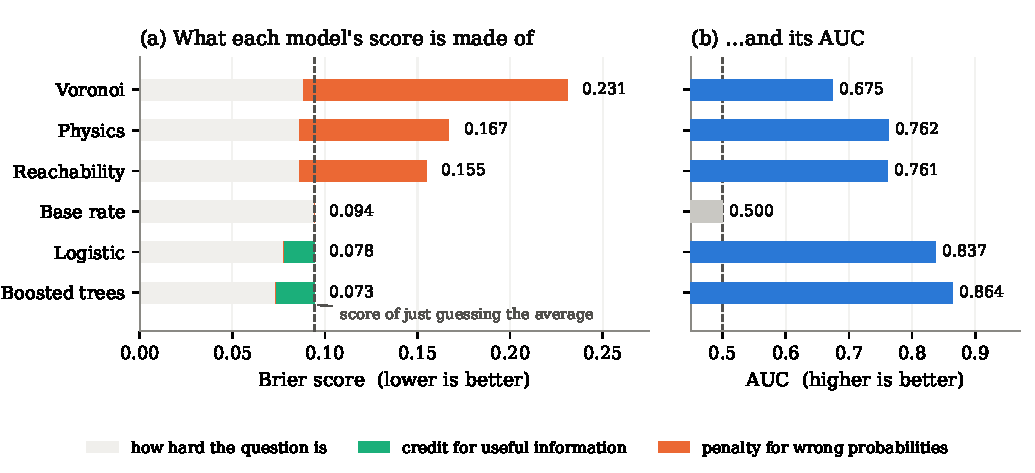
\includegraphics[width=\textwidth]{figures/fig04_decomposition.pdf}
  \caption{\textbf{Where each model's score comes from, and how it looks on AUC.}
  (a)~The Brier score decomposed: difficulty of the question, minus credit for
  useful information, plus penalty for wrong probabilities. Everything to the
  right of the dashed line is worse than guessing the average. (b)~The same
  models ranked by AUC. The physics and reachability models sit comfortably above
  chance in~(b) while being the second- and third-worst forecasts in~(a).}
  \label{fig:decomposition}
\end{figure}

\subsection{Comparison against fitted baselines}

Table~\ref{tab:paired} gives paired cluster-bootstrap differences in Brier score
against M3, computed on identical test arrivals. Positive values favour the
baseline.

\begin{table}[h]
\centering
\small
\caption{Paired differences in Brier score against the penalised logistic
baseline (M3). ``Baseline'' means the baseline wins.}
\label{tab:paired}
\begin{tabular}{lcc}
\toprule
Model & $\Delta$Brier vs M3 [95\% CI] & Verdict \\
\midrule
M1 Voronoi          & $+0.153$ [0.142, 0.163]     & baseline \\
M2 Physics          & $+0.089$ [0.082, 0.096]     & baseline \\
M2a Reach.\ sigmoid & $+0.077$ [0.072, 0.082]     & baseline \\
M0 Base rate        & $+0.017$ [0.015, 0.019]     & baseline \\
M4 GBM              & $-0.005$ [$-0.005$, $-0.004$] & model \\
\bottomrule
\end{tabular}
\end{table}

A penalised logistic regression, given \emph{exactly} the state the physics model
receives, is decisively better. Two further observations follow. M2 and M2a
differ by 0.012 Brier while both sit 0.08--0.09 above M3, so the competing-risks
dynamics add little beyond a monotone squash of a time-to-point difference ---
most of what M2 does could be done with one fitted parameter. And M2's DSC
(0.008) is less than half M3's (0.017), so the gap is not only scale: the physics
model also carries less information about which arrivals differ.

\subsection{Where the error concentrates}

All 47 pre-registered strata show FDR-adjusted evidence of miscalibration
($\alpha = 0.05$). Every directional prediction registered in advance is
supported.

\begin{table}[h]
\centering
\small
\caption{Selected strata for the physics model (M2). MCB is the
cross-fitted miscalibration term; slope is the calibration slope, where 1.0 would
be honest.}
\label{tab:strata}
\begin{tabular}{lrrr}
\toprule
Stratum & $n$ & MCB & Slope \\
\midrule
Attacking third              & 12{,}161 & 0.158 & 0.273 \\
Middle third                 & 20{,}448 & 0.057 & 0.359 \\
Defensive third              & 8{,}258  & 0.031 & 0.324 \\
\addlinespace
Pass 0--10\,m                & 10{,}790 & 0.070 & 0.447 \\
Pass 20--30\,m               & 7{,}484  & 0.098 & 0.264 \\
Pass 30--45\,m               & 3{,}124  & 0.126 & 0.190 \\
Pass 45\,m$+$                & 987      & 0.156 & 0.092 \\
\addlinespace
Pressure: 0 opponents        & 12{,}679 & 0.075 & 0.306 \\
Pressure: 3$+$ opponents     & 1{,}705  & 0.114 & 0.336 \\
\addlinespace
\textbf{Attacking fifth, central} & 2{,}175 & \textbf{0.292} & 0.185 \\
\bottomrule
\end{tabular}
\end{table}

Miscalibration is five times worse in the attacking third than the defensive
third, rises monotonically with pass length, and is worst of all in the central
attacking fifth --- the penalty area, where the mean forecast is 0.34 against an
observed rate of 0.84. This is precisely the region where space-creation and
possession-value metrics are most used and most consequential.
Figure~\ref{fig:breaks} maps it.

\begin{figure}[t]
  \centering
  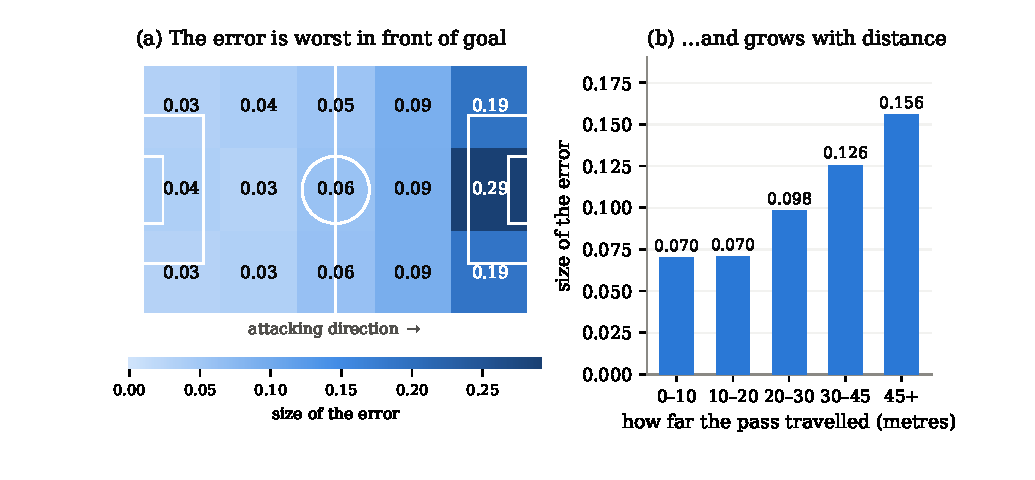
\includegraphics[width=\textwidth]{figures/fig05_where_it_breaks.pdf}
  \caption{\textbf{The error is not spread evenly.} (a)~Miscalibration by pitch
  zone for the physics model, attacking left to right. The worst cell is the
  central attacking fifth --- the penalty area --- at nearly ten times the error
  of the defensive flanks. (b)~The same statistic by pass length: it more than
  doubles from short passes to long ones.}
  \label{fig:breaks}
\end{figure}

\subsection{How much of it is the camera?}

Calibration improves monotonically with the fraction of the frame observed
(Table~\ref{tab:completeness}, Figure~\ref{fig:observability}). Destinations
outside the visible area are far worse (MCB 0.145, slope 0.167, $n = 8{,}565$)
than those inside it (0.064, 0.390, $n = 32{,}302$).

\begin{table}[h]
\centering
\small
\caption{Miscalibration of the physics model by how much of the frame the camera
recorded.}
\label{tab:completeness}
\begin{tabular}{lrrr}
\toprule
Frame completeness & $n$ & MCB & Slope \\
\midrule
$<60\%$    & 11{,}040 & 0.095 & 0.221 \\
60--75\%   & 12{,}277 & 0.086 & 0.300 \\
75--90\%   & 13{,}104 & 0.076 & 0.385 \\
$90\%+$    & 4{,}446  & 0.049 & 0.556 \\
\bottomrule
\end{tabular}
\end{table}

\begin{figure}[t]
  \centering
  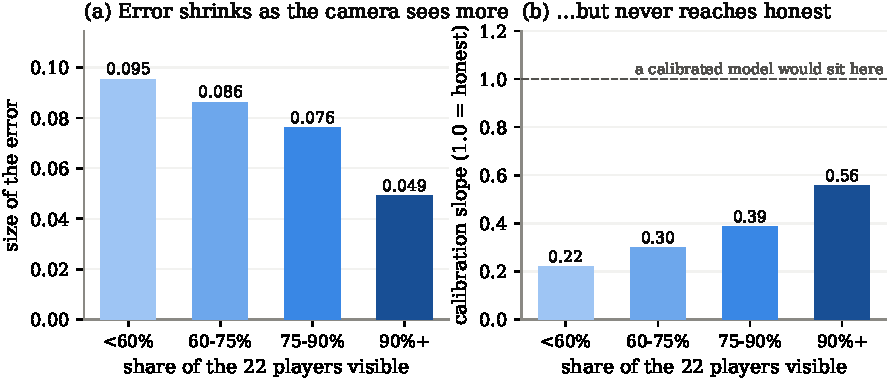
\includegraphics[width=\textwidth]{figures/fig06_observability.pdf}
  \caption{\textbf{Better observation helps, and is not enough.} (a)~The error
  falls by roughly half as the share of visible players rises. (b)~The
  calibration slope rises towards 1.0 but stops at 0.56 even in the best-observed
  frames --- values below 1.0 mean the probabilities are spread too far towards 0
  and 1. Note that better-observed frames are not a random subsample, so this is
  an association, not a causal decomposition.}
  \label{fig:observability}
\end{figure}

Restricting to near-complete frames \emph{with} a visible destination gives
MCB 0.045 and slope 0.571, against 0.081 and 0.306 overall --- so roughly
\textbf{45\% of the measured miscalibration is attributable to incomplete
observation and 55\% survives it}. Even when the camera sees nearly everything,
the velocity-free model remains badly overconfident while its AUC rises to 0.86:
the same divergence, at better data quality.

This decomposition is \textbf{suggestive, not causal}. High-completeness frames
are not a random subsample --- the ball is more often in crowded central areas ---
so the comparison confounds observability with the kind of situation observed.

\subsection{Selection}
\label{sec:selection}

\begin{plainbox}[A negative result, reported as one]
\small
The reweighting arm of the analysis \textbf{failed its own diagnostics, and we
report it as failed rather than reporting the number it produced.}
\end{plainbox}

A classifier separating chosen from proposed destinations achieves AUC 0.972:
passers select their targets very strongly, which confirms the premise that
selection is a real threat. But the overlap diagnostics are damning.
\textbf{52.6\% of observed arrivals lie outside the support of the candidate
distribution}; the top 1\% of weights carry 33\% of the mass; the largest weight
is 521; and the effective sample size collapses from 48{,}268 to 7{,}753 (16\%)
under the trimmed, stabilised weights the analysis actually uses --- 1{,}525, or
3\%, before trimming. Under those conditions the reweighted estimate (MCB 0.127
against an unweighted 0.085) is extrapolation, not correction, and we do not
interpret it.

Stratification is more informative. Table~\ref{tab:strat} splits the test fold by
quintile of the selection score, where stratum~0 holds the destinations a passer
would be least likely to choose.

\begin{table}[h]
\centering
\small
\caption{Miscalibration by how typical the destination is. The model is worst
exactly where a practitioner would most want to consult it.}
\label{tab:strat}
\begin{tabular}{lrrrr}
\toprule
Stratum & $n$ & Base rate & Mean forecast & MCB \\
\midrule
0 (least typical) & 9{,}654 & 0.790 & 0.507 & 0.148 \\
1                 & 9{,}653 & 0.896 & 0.612 & 0.157 \\
2                 & 9{,}654 & 0.932 & 0.782 & 0.065 \\
3                 & 9{,}653 & 0.959 & 0.865 & 0.039 \\
4 (most typical)  & 9{,}654 & 0.969 & 0.906 & 0.022 \\
\bottomrule
\end{tabular}
\end{table}

The model is worst on the destinations players choose least often, by a factor of
roughly seven. The headline figure of 0.081 is therefore a weighted average
dominated by routine passes, and it \emph{understates} the error in the unusual
situations where a control model would most plausibly be consulted.

\textbf{The strongest available identification strategy could not be run.} The
proposal's primary answer to selection was a quasi-exogenous subsample ---
deflections, clearances and second balls, which arrive where nobody aimed. This
corpus contains none: only pass events carry both a start and an end location.
That is a real limitation, and its absence is why the sensitivity analysis
carries more weight here than intended.

That sensitivity analysis is reassuring. Modelling unmeasured selection as a
multiplicative bias $\Gamma$ on the outcome odds among observed arrivals, in the
style of \citet{rosenbaum1983propensity}, MCB remains 0.039 even at
$\Gamma = 3$ --- an implausibly strong assumption about what passers know and the
state vector does not. \textbf{No tipping point exists within the range
examined}: the finding is not explicable by unmeasured selection of any plausible
magnitude.

\subsection{Does it transport, and can it be fixed?}

\begin{table}[h]
\centering
\small
\caption{Leave-one-competition-out transportability. ``Penalty for crossing'' is
the difference between the two preceding columns.}
\label{tab:transport}
\begin{tabular}{lrrr}
\toprule
Model & MCB within competition & MCB across competitions & Penalty for crossing \\
\midrule
M2 Physics  & 0.085  & 0.083  & $\mathbf{-0.002}$ \\
M3 Logistic & 0.0010 & 0.0011 & $+0.0001$ \\
M4 GBM      & 0.0006 & 0.0004 & $-0.0002$ \\
\bottomrule
\end{tabular}
\end{table}

Crossing a competition boundary costs essentially nothing, \textbf{including the
men's-to-women's boundary}, despite base rates differing materially (0.909,
0.921, 0.859). The miscalibration is structural, not local: the model is equally
wrong everywhere. That is a stronger and more useful claim than being wrong on
one league.

It follows that one fix travels. A recalibration map fitted on two competitions
and applied to a third, unseen one removes \textbf{97--99\%} of the physics
model's measured miscalibration (isotonic 98.9\% on average, worst case 98.6\%;
beta 98.6\%/98.3\%; Platt 97.4\%/96.4\%). On the main match-level split, all
three maps drive MCB from 0.081 to within 0.001 of zero.
Figure~\ref{fig:transport} shows both halves of the result.

\begin{figure}[t]
  \centering
  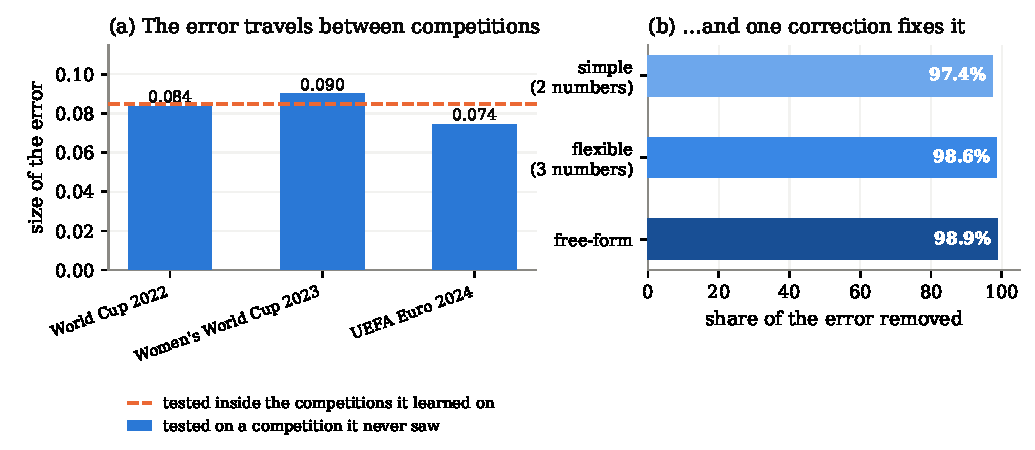
\includegraphics[width=\textwidth]{figures/fig07_transport.pdf}
  \caption{\textbf{The defect travels, and so does the repair.} (a)~Holding out
  each competition in turn changes the error hardly at all relative to testing
  inside the competitions the map was built on --- including across the
  men's/women's boundary. (b)~A correction fitted on two competitions and applied
  to the third removes almost all of the error, and a two-parameter map is
  nearly as good as a free-form one.}
  \label{fig:transport}
\end{figure}

The model's \emph{ordering} of situations is therefore sound; only its scale is
wrong. The defect is repairable downstream by a two- or three-parameter map that
a practitioner can fit once and deploy --- a deflating result, and a useful one.

\subsection{Does the conclusion survive the definition of control?}
\label{sec:construct}

The study imposes an operational definition on an undefined construct. The
pre-registered rule was that a conclusion which flips across the sweep would be
reported as flipping. It does not flip.

\begin{table}[h]
\centering
\small
\caption{Sensitivity to the outcome definition and horizon, physics model (M2).}
\label{tab:construct}
\begin{tabular}{llrrrrr}
\toprule
Definition & Horizon & Base rate & Censored & MCB & Slope & AUC \\
\midrule
Control at horizon & 0.25\,s & 0.917 & 0.6\% & 0.088 & 0.306 & 0.772 \\
Control at horizon & 1.0\,s  & 0.911 & 1.2\% & 0.084 & 0.300 & 0.768 \\
Control at horizon & 3.0\,s  & 0.883 & 2.9\% & 0.070 & 0.278 & 0.748 \\
First touch        & ---     & 0.918 & 0.0\% & 0.088 & 0.304 & 0.772 \\
Retained sequence  & ---     & 0.912 & 1.2\% & 0.084 & 0.303 & 0.770 \\
Possession at 5\,s & ---     & 0.855 & 1.9\% & 0.064 & 0.219 & 0.705 \\
\bottomrule
\end{tabular}
\end{table}

Across six horizons and four outcome definitions, MCB stays in [0.064, 0.088] and
the slope in [0.219, 0.306]. The conclusion is not an artefact of the horizon.
Notably, the \textbf{first-touch} definition --- the closest observable proxy for
the reachability construct that dominant-region models actually compute --- gives
MCB 0.088, no better than the possession definition. The models are not merely
being scored against the wrong target.

Censoring rises from 0.6\% to 2.9\% as the horizon lengthens. Since fouls cluster
in contested areas, a longer horizon buys construct breadth at the cost of a more
selected sample; the effect is small at these rates but is reported rather than
assumed away.

% ===========================================================================
\section{Practical implications}
% ===========================================================================

\subsection{Possession value is understated by more than a quarter}

Propagating raw and recalibrated control values through a linear
expected-possession-value construction over the 40{,}867 test arrivals gives
Table~\ref{tab:epv}.

\begin{table}[h]
\centering
\small
\caption{Expected possession value computed from raw and recalibrated control
values, at a loss discount of 0.35.}
\label{tab:epv}
\begin{tabular}{lrr}
\toprule
Control variant & Mean EPV & Total EPV \\
\midrule
Raw      & 0.559 & 22{,}844 \\
Platt    & 0.774 & 31{,}613 \\
Isotonic & 0.773 & 31{,}581 \\
Beta     & 0.773 & 31{,}576 \\
\bottomrule
\end{tabular}
\end{table}

Aggregate possession value computed from raw control values is \textbf{28\%
lower} than from calibrated ones. This is the accumulation argument made
concrete: because EPV is linear in $C$, a calibration error with a consistent
sign does not average out across a season --- it compounds.

\subsection{A third of pass recommendations change}

\begin{table}[h]
\centering
\small
\caption{Effect of recalibration on threshold-based pass recommendations.}
\label{tab:decisions}
\begin{tabular}{lrrr}
\toprule
Threshold & Recommendations changed & Accuracy raw & Accuracy recalibrated \\
\midrule
0.50 & 25.2\%          & 0.762 & 0.895 \\
0.60 & 30.6\%          & 0.727 & 0.895 \\
0.70 & \textbf{36.0\%} & 0.680 & 0.892 \\
0.80 & 24.0\%          & 0.622 & 0.792 \\
\bottomrule
\end{tabular}
\end{table}

\begin{figure}[t]
  \centering
  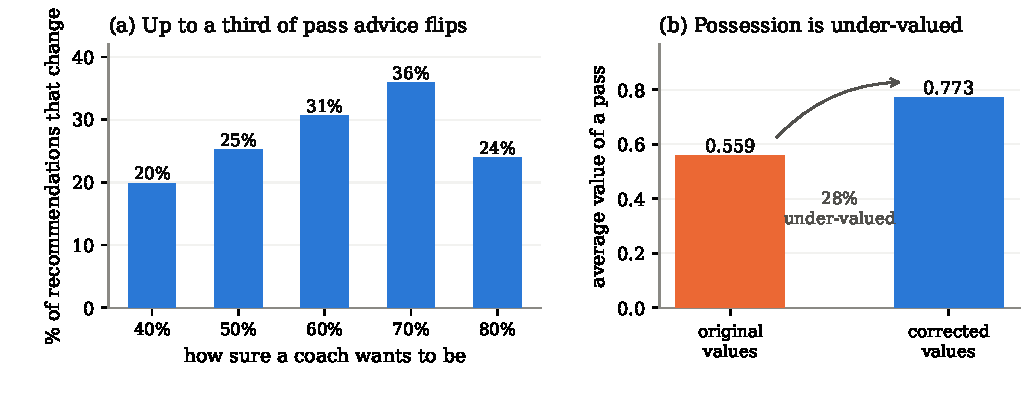
\includegraphics[width=\textwidth]{figures/fig08_downstream.pdf}
  \caption{\textbf{What the miscalibration costs in football terms.} (a)~The
  share of pass recommendations that change once the control values are
  corrected, as a function of how sure a coach wants to be before playing the
  pass. (b)~Aggregate possession value over the test fold, before and after
  correction.}
  \label{fig:downstream}
\end{figure}

\subsection{But read the mechanism carefully}

Recalibration improves net benefit \citep{vickers2006decision} at 90 of 91
thresholds, and doubles the range over which the model beats the best default
policy (from 15 thresholds to 31). It is tempting to conclude that recalibration
makes the model better at football. It does not.

Every map used here is monotone, so AUC is unchanged to machine precision: the
model's \emph{ranking} of arrivals is identical before and after. What
recalibration restores is the \textbf{meaning of the threshold}. A practitioner
who sets a cut-off from a stated risk appetite --- ``attempt the pass when
control probability exceeds 0.7'' --- is, with the raw forecast, actually
operating at a far stricter point than intended, because a raw 0.7 corresponds to
an observed rate near 0.9. A practitioner who instead tuned their threshold
empirically on the raw forecasts would already be getting the same decisions.

So the honest statement is narrower than ``recalibration improves decisions'':

\begin{plainbox}[The correct reading]
\small
\textbf{Miscalibration corrupts any use of the value that is not purely
ordinal} --- summing, multiplying, integrating, or comparing against an
externally chosen threshold. Purely ordinal uses, such as ranking a player's
passing options against each other, are unaffected.
\end{plainbox}

% ===========================================================================
\section{Limitations}
\label{sec:limits}
% ===========================================================================

\paragraph{This does not test full-tracking pitch-control models.}
The single most important limitation. No model here has velocity, and velocity is
the primary input the physics formulations were designed around. The results
bound what those models do under degraded data; they do not measure what they do
under the data they were built for. The observability analysis suggests
observability explains under half of the error, but that decomposition is not
causal, and the velocity component cannot be separated at all on this corpus.

\paragraph{Construct mismatch is a live objection.}
Dominant-region models answer ``who arrives first''; we score against ``who ends
up with the ball''. A defender of these models could argue we are scoring them
against a target they never claimed. Two responses. First, the downstream
literature does use these fields for the second question; if they answer only the
first, that invalidates the downstream uses rather than excusing the models.
Second, and more directly: under the first-touch definition, the closest
observable proxy for reachability, MCB is 0.088 --- no better. The mismatch does
not explain the result.

\paragraph{The selection analysis is incomplete.}
The quasi-exogenous subsample could not be constructed, the reweighting failed
its overlap diagnostics, and we are left with stratification and a sensitivity
bound. The bound is strong (no tipping point below $\Gamma = 3$), but it is a
bound, not identification.

\paragraph{Observational data cannot identify control where the ball never
arrives.} Our conclusions extend to realised arrivals. That is also where every
downstream application operates, so the limitation is narrower than it sounds ---
but the full field's claims remain untested and, on observational data,
untestable.

\paragraph{Three competitions, two of them elite men's tournaments.}
Transportability held across the men's/women's boundary, which is evidence
against population-specificity, but youth and lower-division football are
untested and the locomotion assumptions have less reason to hold there.

\paragraph{Parameter sensitivity was not exhausted.}
The arrival-time uncertainty $\sigma$ governs the field's sharpness directly, and
our ablations on smaller corpora showed it moving the calibration slope by more
than the difference between models. A $\sigma$ fitted to outcomes would likely
improve M2 substantially --- which is itself the point: a parameter that must be
fitted to outcomes is not physics.

% ===========================================================================
\section{Conclusion}
% ===========================================================================

On 137{,}545 realised ball arrivals, velocity-free pitch-control values are not
calibrated probabilities. The physics-based model scores worse than forecasting
the base rate while discriminating well above chance; its calibration slope is
0.306; a penalised logistic regression given identical inputs is decisively
better. The error concentrates in the attacking third, grows with pass length,
worsens where the camera sees less, and is seven times larger on the destinations
players choose least often. It transports unchanged across three competitions and
across the men's/women's boundary, and it survives every horizon and outcome
definition we pre-registered.

It is also almost entirely removable. A recalibration map fitted on two
competitions strips 97--99\% of it from a third. The ordering these models
produce is sound; the numbers attached to that ordering are not.

The practical recommendation is therefore specific rather than dismissive.
Pitch-control fields remain useful for ranking. They should not be summed,
integrated, multiplied by positional values, or compared against externally
chosen thresholds without recalibration --- and on this evidence a single global
map suffices to make them fit for those uses.

Whether the same holds for full-tracking implementations is the obvious next
question, and it needs a corpus this study did not have.

% ===========================================================================
\appendix
\section{Reproduction}
% ===========================================================================

\begin{verbatim}
pip install -r requirements.txt && pip install -e .
python scripts/09_validate_instrument.py       # validate the estimator first

for spec in "43 106" "55 282" "72 107"; do set -- $spec
  python scripts/fetch_data.py --source statsbomb_open --accept-terms \
      --competition $1 --season $2 --with-360
done

SRC="--source statsbomb_open"

python scripts/03_main_analysis.py         $SRC --n-boot 1000
python scripts/04_subgroup_analysis.py     $SRC
python scripts/05_selection_analysis.py    $SRC --max-matches 60
python scripts/06_downstream_analysis.py   $SRC
python scripts/11_transportability.py      $SRC
python scripts/12_construct_sensitivity.py $SRC --max-matches 64
python scripts/14_make_figures.py          # rebuild every figure
\end{verbatim}

Every results directory carries a manifest recording the git revision, package
versions, and a hash of the configuration. Protocol, hypotheses and subgroups are
in \texttt{docs/proposal.md}; dataset verification in
\texttt{docs/data\_sources.md}. \texttt{scripts/13\_verify\_paper.py} re-checks
every numeric claim in this paper against the files in \texttt{results/}.

\bibliographystyle{plainnat}
\bibliography{references}

\end{document}
